\section{M2M Applications, Classifications and QoS requirements}
\label{sec:overview-m2m-app-class}
M2M communication is expected to be an integrated part of the future wireless networks. For example, a future LTE network will see the coexistence of MTC and HTC as what is shown in Fig.~\ref{fig:mtc-in-lte-use-case}. The types of M2M applications are various, including but not limited to security, intelligent transport system, payment, health, remote maintenance/control, metering, consumer devices bicycle sharing system~\cite{OECD/Report}, logistics application, insurance~\cite{OECD/Report}. In Tab.~\ref{tab:MTC applications categorization}, we resume the M2M applications listed by 3GPP.
\begin{figure}[h]
	\centering
	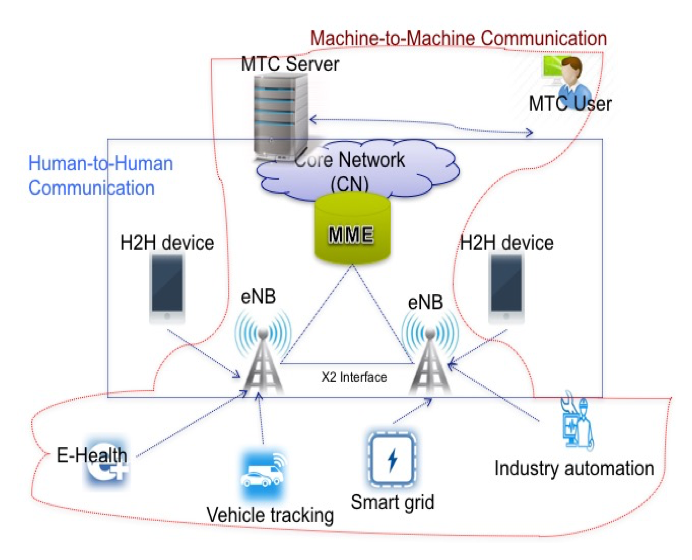
\includegraphics[width=0.7\linewidth, height=7cm]{Chapter2/Figures/MTC_use_case}
	\caption{Coexistence of MTC and HTC in the future LTE networks}
	\label{fig:mtc-in-lte-use-case}
\end{figure}

Given that M2M applications are so various, it is impossible to develop a unique platform to support all these applications in an economical way. For example, the metering device is desired to be simple but the video surveillance device needs different and powerful codec, different protocols and should have different radio capabilities. If only one solution or hardware platform is adopted for all the services, the consequence is a MTC machine with the high complexity, which is like a smart phone today~\cite{ChenY10machine}. Thus, it is important to classify the existing M2M applications and propose improvement according to different requirements. In addition, an appropriate M2M classification helps identify QoS features and other works. 
%Borges et al.~\cite{borges2014survey} give a detailed classification for Wireless Sensor Network (WSN) applications, which is useful for the classification of cellular M2M applications.  
In this section, we present all classification schemes found in the literature, each of which may serve for specific research purpose. 
%\begin{table}[H]
%%	\centering
%	\caption{MTC applications categorization (Non-exhaustive) according to \cite{3GPP/service-requirement}\cite{GhavimiF2015}\cite{mehmood2015mobile}}
%	\label{tab:MTC applications categorization}		
%	\resizebox{0.7\linewidth}{!}{%
%		\begin{tabular}{@{}ll@{}}
%			\toprule
%			service area                                                            & MTC applications                   \\ \midrule
%			\multirow{4}{*}{Security}                                               & Surveillance systems               \\
%			& Backup for landline                \\
%			& Control of physical access         \\
%			& Car/driver security                \\ \midrule
%			\multirow{7}{*}{Intelligent Transport system}                                      & Fleet management                   \\
%			& Order management                   \\
%			& Pay as you drive                   \\
%			& Assess tracking                    \\
%			& Navigation                         \\
%			& Traffic information                \\
%			& Road tolling                       \\ \midrule
%			\multirow{3}{*}{Payment}                                                & Point of sales                     \\
%			& Vending machine                    \\
%			& Gaming machines                    \\ \midrule
%			\multirow{4}{*}{Health}                                                 & Monitoring vital signals           \\
%			& Supporting the aged or handicapped \\
%			& Web access telemedicine points     \\
%			& Remote diagnostics                 \\ \midrule
%			\multirow{5}{*}{Remote maintenance/control}                             & Elevator control                   \\
%			& Lighting                           \\
%			& Pumps                              \\
%			& Industrial automation              \\
%			& Vehicle diagnostics                \\ \midrule
%			\multirow{4}{*}{Metering}                                               & Power/Gas/Water                    \\
%			& Heating                            \\
%			& Grid control                       \\
%			& Industrial metering                \\ \midrule
%			Consumer devices                                                        & Digital photo frame                \\
%			& E-book                             \\ \midrule
%			\begin{tabular}[c]{@{}l@{}}Other futuristic\\ applications\end{tabular} & Information ambient society        \\
%			& Robotic applications               \\
%			& Environment monitoring             \\ \bottomrule
%		\end{tabular}
%		}
%\end{table}

% % % Long table version. longtable environment cannot be placed into box.
\begin{center}
	\begin{longtable}{ll}
		\caption{MTC applications categorization (Non-exhaustive) according to \cite{3GPP/service-requirement}\cite{GhavimiF2015}\cite{mehmood2015mobile}} 
		\label{tab:MTC applications categorization}		\\
		\toprule
		service area                                                            & MTC applications                   \\ \midrule
		\multirow{4}{*}{Security}                                               & Surveillance systems               \\
		& Backup for landline                \\
		& Control of physical access         \\
		& Car/driver security                \\ \midrule
		\multirow{7}{*}{Intelligent Transport system}                                      & Fleet management                   \\
		& Order management                   \\
		& Pay as you drive                   \\
		& Assess tracking                    \\
		& Navigation                         \\
		& Traffic information                \\
		& Road tolling                       \\ \midrule
		\multirow{3}{*}{Payment}                                                & Point of sales                     \\
		& Vending machine                    \\
		& Gaming machines                    \\ \midrule
		\multirow{4}{*}{Health}                                                 & Monitoring vital signals           \\
		& Supporting the aged or handicapped \\
		& Web access telemedicine points     \\
		& Remote diagnostics                 \\ \midrule
		\multirow{5}{*}{Remote maintenance/control}                             & Elevator control                   \\
		& Lighting                           \\
		& Pumps                              \\
		& Industrial automation              \\
		& Vehicle diagnostics                \\ \midrule
		\multirow{4}{*}{Metering}                                               & Power/Gas/Water                    \\
		& Heating                            \\
		& Grid control                       \\
		& Industrial metering                \\ \midrule
		Consumer devices                                                        & Digital photo frame                \\
		& E-book                             \\ \midrule
		\begin{tabular}[c]{@{}l@{}}Other futuristic\\ applications\end{tabular} & Information ambient society        \\
		& Robotic applications               \\
		& Environment monitoring             \\ \bottomrule
	\end{longtable}
\end{center}


%%%%%%%%%%%%%%%%%%%%%%%%%%%%%%%%%%%%%%%%%%%%%%%%%%%%%%%%%%%%%%%%%%%%%%%%%%%%%%%%%%%%%%%%%%%%%%%%%%%%%%%%%%%%%%%%%%%%%%%%%%%%%%%%%%%%%%%%%%%%%%%%%%%%%%%%%%%%%%%%%%%%%%%%%%%%%%%%%%%%%%%%%%%%%%%%%%%%%%%%%%%






%Maybe in the end, we could resume all discussed cellular M2M applications %in a table. like table 1 in \cite{WuTJHJ11}

% 3GPP R1-120056, “Analysis on traf􏰐c model and characteristics for MTC and text proposal,” Technical Report, TSG-RAN Meeting WG1#68, Dresden, Germany, Feb. 2012. [Online]. Available: http://www.3gpp.org ====》 研究MTC traffic特点的

%LOLA Deliverable 3-4 – M2M Traf􏰐c Model, ICT-LOLA Project Deliverable (Achieving LOw-LAtency in Wireless Communications), 2012. [Online]. Available: http://www.ict-lola.eu 也是研究 MTC traffic特点的。(未读)


% SInce we use a use case-driven approach to anaylize QoS requrements for M2M applications..we need to do an appropriate M2M application classfication.
% present QoS class in detail (the principle is first to find some references in which the same job is done, if no, classify ourself.)
% QoS may be in form of RRT(delay), pakcet loss ration(quantifying reliability)
%The experiment results \cite{FirstLook12} show that M2M traffic suffer from a higher packet loss ration compared to that of smartphone. The possible reasons may be either the poor 
%deployemet location or the lack of user interface that clearly displays cellular singal strength.
\subsection{Classification according to reliability and quantity of connected machines }
According to reliability and quantity of connected machines, 
the project METIS divides M2M applications into two categories: mMTC and uMTC~\cite{METIS15_concept}. 
mMTC refers to massive MTC and provides connectivity for a large number of cost and energy-constrained devices.
Sensor and actuator deployments can be in a wide-area for surveillance and area-covering measurements, but also co-located with human users, as in body-area networks. 
The main attribute of this service is the massive number of connected devices, where the required rates decrease as the number of devices grows significantly. 
uMTC addresses the needs for ultra-reliable, time-critical services, e.g., V2X (Vehicle-to-Vehicle/Infrastructure) applications and industrial control applications. 
Both examples require reliable communication and V2X additionally requires fast discovery and communication establishment. 
The main attribute is high-reliability, while the number of devices and the required data rates are relatively low. 
\subsection{Classification according to the level of mobility and dispersion}
According to the level of mobility and dispersion, M2M applications also could be categorized into four categories: dispersed and fixed application, dispersed and mobile application, concentrated and fixed application, concentrated and mobile application~\cite{OECD/Report}. 
The dispersion refers to the area that the M2M devices are spread out over. 
The mobility measures whether the device is stationary or whether it needs to move around. 
The typical example for dispersed and fixed application is smart grid where sensors are deployed in a large scale at a fixed location. 
Logistic applications are representative for dispersed and mobile application. 
For example, the sensors to track the cargo in the container may spread and move anywhere.
Fig.~\ref{fig:OECD-M2M-app-classification} shows the result of classification for some typical M2M applications according to this criterion.
\begin{figure}[!th]
	\centering
	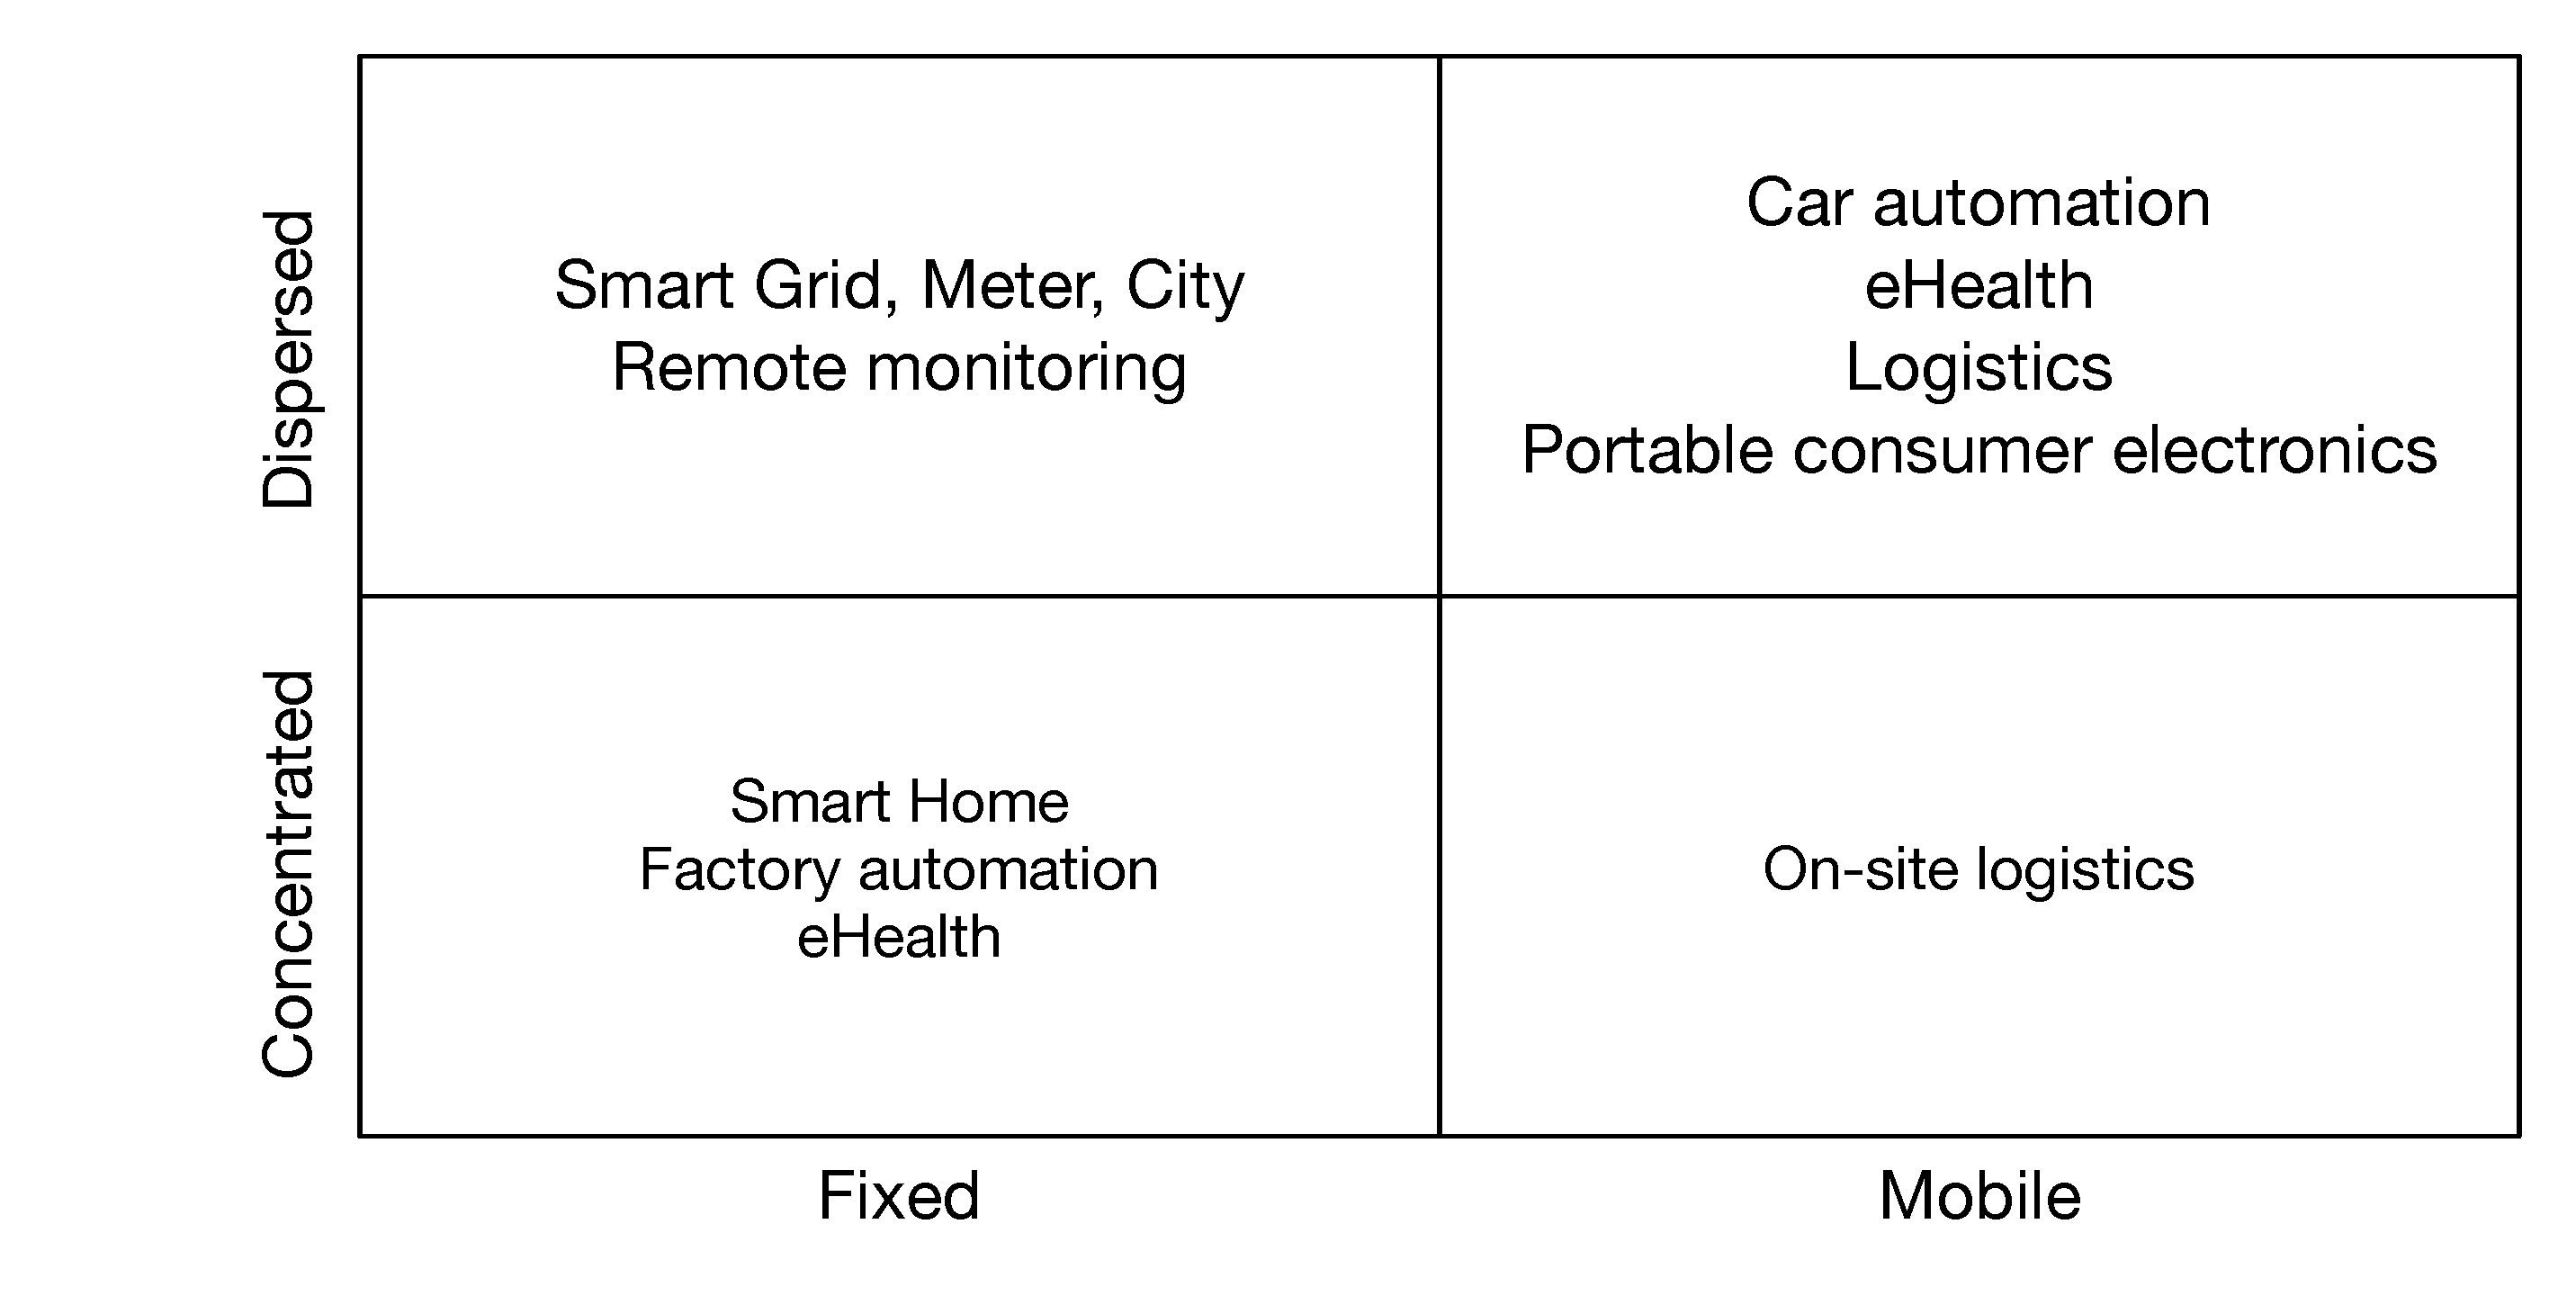
\includegraphics[width=0.7\linewidth]{OECD-M2M-app-classification}
	\caption{M2M applications taxonomy by mobility and dispersion. Source: \cite{OECD/Report}}
	\label{fig:OECD-M2M-app-classification}
\end{figure}
\subsection{Classification according to delay tolerance level}
According to delay tolerance level, M2M applications can be divided into $4$ classes: Class 1 (Elastic applications), Class 2 (Hard real-time applications), Class 3 (Delay-adaptive applications), Class 4 (Rate-adaptive applications~\cite{KanZheng12}. The Class 1 applications are generally rather tolerant of delays, for example, file downloading of remote MTC devices from MTC servers. The Class 2 applications need their data to be served within a given delay constraint. The typical example of class 2 application is vehicle and asset tracking. 
Similar to class 2, the class 3 applications are usually delay sensitive, but most of applications of class 3 can be made rather tolerant of occasional delay-bound violation and dropped packets. 
The class 4 applications adjust their transmission rates according to available radio resources while maintaining moderate delays. 
\subsection{Classification according to data reporting mode}
According to data reporting mode, M2M applications are classified into five categories~\cite{al2004routing}\cite{Costa14}\cite{borges2014survey}: Time-driven, Query-driven, Event-driven, Continuous based and hybrid-driven. Time-driven M2M applications refer to those applications where machines periodically turn on their sensors and transmitters to transmit the collected data. Query-driven applications reply to
certain instructions from MTC servers by transmitting data. This type of applications allows packet omissions, as adjacent data reports usually contain redundant information. Event-driven applications react to certain critical query or event. Normally, applications fall into this category when they use priority alarm messages (PAM). Continuous based M2M applications make the devices send their data continuously to the remote server at a prespecified rate. Hybrid-driven is a combination of aforementioned types.

\subsection{QoS feature for typical M2M applications}
In Tab.~\ref{tab:QoS feature and M2M application}, a QoS requirement table in terms of data rate, latency and message priority is given for some representative cellular M2M applications, based on different references found in the literature. It should be noted that in Tab.~\ref{tab:QoS feature and M2M application}, we give only indicative values.
\begin{table*}[!h]
	\centering
	\caption{Typical M2M applications and their QoS Requirements}
	\label{tab:QoS feature and M2M application}
	\resizebox{0.95\textwidth}{!}{%
		\begin{tabular}{@{}llll@{}}
			\toprule
			M2M service              & Data rate                                                & Latency                                       & Priority \\ \midrule
			Surveillance system      & $64.000$ bits/s\cite{ratasuk12coverage}                  & small                                         & Medium   \\
			Urgent notification      & small                                                    & less than 1 s                                 & High     \\
			Fleet management         & less than 500 bytes                                      & very small                                    & High     \\
			Pay as you pay           & small                                                    & very small                                    & High     \\
			Smart metering           & 500-1000 bytes per message                               & 15 sec - 15 min \cite{3GPP/TSG-RAN/R2-102340} & Low      \\
			Grid automation          & 10-100 kps\cite{poncela2015m2m}                          & 0.1-2 sec\cite{poncela2015m2m}                & High     \\
			Monitoring vital signals & less than 200 bytes per message \cite{HealthInformatics} & small                                         & High     \\
			Monitoring in emergency  & less than 200 bytes per message \cite{HealthInformatics} & small                                         & High     \\
			Industrial automation    & small                                                    & less than 5 ms \cite{ratasuk2015recent}       & High     \\
			Vending machine control  & small                                                    & small                                         & Medium   \\ \bottomrule
		\end{tabular}
	}
\end{table*}

%------------------------------------正文开始----------------------------------------------